% ====================================================================
%+
% NAME:
%    youngstars.tex
%
% CHAPTER:
%    variables.tex
%
% ELEVATOR PITCH:
%-
% ====================================================================

\section{Discovery and Characterization of Young Stellar Populations}
\def\secname{youngstars}\label{sec:\secname}

\credit{phartigan},
\credit{CJohnsKrull},
\credit{pmmcgehee}

\subsection{Introduction}

All young stars exhibit some form of
photometric variability, and these variations hold the key
to understanding the diverse physical processes present at starbirth
such as mass accretion events from circumstellar disks, presence of
warps in envelopes, creation of new knots in stellar jets,
evolution of stellar angular momenta, starspot longevity and cycles,
and the frequency and strength of flares.
With the proper cadences and filter choices,
LSST will make a significant impact in our understanding of all
these phenomena simply by providing large enough samples to allow
us to relate these aspects of the young stars and their environments
to stellar properties such as mass, age, binarity,
and their location within their nascent dark clouds in a statistically
significant manner.

Low-mass ($\lessim 1.5 M_{\odot}$) pre-main-sequence stars separate
into two main categories, depending upon whether or not an optically thick
dusty circumstellar disk exists in the system: young stars without dusty
inner disks are known as `weak-lined T Tauri stars' (wTTs), while those
that have inner dusty disks are called `classical T Tauri stars'.
The nature of the variability in young stars changes with evolutionary status.
In cTTs, variability is primarily caused by unsteady mass infall from circumstellar disks
onto their stars, and from periodic extinction events that unfold as dense
clumps or disk warps circle the star in Keplerian orbits.
Once the disks become optically thin, variability in the wTTs phase
is dominated by small-amplitude (typically $\sim$ 0.1 mag)
quasi-periodic variations that arise
from cool star spots, though active regions that generate X-rays in
these objects undoubtedly produce optical flares as well.

At the extreme end of cTTs phenomena, rare massive
outbursts of up to 6 magnitudes with decay times between several months
to over a hundred years in pre-main-sequence stars (EX Ori's \citep{herbig01}
and FU Ori's \citep{hartmann96})
are of great interest to studies of disk accretion because they indicate the onset of
a major disk instability. Only a handful of such systems have been found, and LSST
will easily detect any new ones.  In addition to triggering
follow-up observations, LSST will define the first population
constraints on the duration of high states, particularly for the shorter-lived
versions of these eruptive variables.

Obtaining rotation periods for large numbers of pre-main-sequence stars is the only way to
quantify how angular momenta of young stars vary with age. For both wTTs and cTTs,
phase-coherence in the rotation periods defines the longevity of star spots, while the
amplitude of the periodic component of the lightcurve constrains the spot coverage (and
temperature if multiple filters are used).  As described in section 8.10.2 in the
LSST Science Book (p298--299), irregular flaring in young stars exists across the entire
$ugrizy$~bandpass of LSST. Flaring can last from minutes to years, with
amplitudes from a few tenths to several magnitudes.  In cTTs, $u$-band fluxes rise during
accretion events, which we can distinguish from extinction events if red magnitudes are
also available. A large accretion event is a signal to observe the system
in the future with other instrumentation to look for evidence of a newly-created
jet knot. In wTTs, Flares also occur in wTTs as a consequence of high chromospheric activity.
Flaring in wTTs is also easiest to monitor at $u$, though the rapid decline of
chromospheric flares requires a rapid cadence to capture correctly.

LSST also provides a potential means to discover new young stars by way of
their variability and colors. One of the challenges in this regard will be to
distinguish young stars from other low-amplitude variable stars in the field.
In that regard we expect that machine-learning techniques that incorporate knowledge of
fluxes in other wavebands as well as the LSST lightcurves and colors will
be an ongoing effort. It is possible that X-ray detections will be more
reliable for detection of new young stars, but LSST will at minimum assist
by identifying non-YSO X-ray sources, and should be a means for discovery
for older pre-main-sequence stars (10 $-$ 30 My range) that have had time
to wander away from the well-known sites of star forming activity that are
typical targets for deep, pointed X-ray surveys.

Galactic star formation regions are largely found at low Galactic
latitudes or within the Gould Belt structure. As such study of young
stars with LSST is closely tied to other science goals concerning the
Milky Way Disk and is subject to the concerns of both crowded field
photometry and the observing cadence along the Milky Way. However, recent
DECam observations at the CTIO 4-m that reached depths similar to those
proposed for LSST show negligible crowding in the optical, and $\lessim$
5\%\ crowding at $z$ in Carina. In this case, extinction in the molecular
clouds helps by significantly lowering the frequency of background contamination.

% --------------------------------------------------------------------

\subsection{Analysis}
\label{sec:\secname:analysis}

{\bf Target Regions}

LSST will allow us to survey the outstanding collection of
star formation regions in the Southern hemisphere, including the closest
such regions ($\rho$ Oph, CrA, Cha~I and Lupus), and the most famous intermediate-mass
(Orion) and massive (Carina) examples.
The closest star forming regions have only low-mass molecular clouds, and each contain
only about 100 young stars. More massive molecular clouds produce both higher
mass stars and more low mass stars. In the Orion Nebula Cluster (d = 414 pc), the number of
identified YSOs is $\sim$ 3000, and we expect $\gtrsim$ 30000 pre-main-sequence
stars in the famous southern star formation region in Carina (2.3 kpc).
LSST will make its greatest impact
when observing the more massive star formation regions, where the amount
of young stars is much higher.

Owing to extinction in the dark clouds,
source confusion will generally not be an issue (as evidenced by typical
deep optical images of such regions), though the large fraction
of pre-main-sequence binaries at all separations ensures that many
lightcurves will be composites of the primaries and secondaries.
More distant star-forming regions will suffer from enhanced foreground
contamination, though it should be possible to eliminate most contaminating
variable stars by combining close inspection of their lightcurves with
colors.

{\bf Metrics:}

{\bf A. Magnitude Limits, Filter Choices}

To quantify YSO studies with LSST, we consider V~927 Tau,
a rather faint, moderately-reddened 0.2 M$_\odot$ young star in the Taurus cloud
as a target goal. Extrapolating this star
to the distance of Carina we have $u$=24.0, $g$=23.0, $r$=20.8, $i$=19.4, and $z$=18.0. For reference,
a typical young star in the Carina X-ray catalog has an $i$-magnitude of 18.
Objects that suffer larger extinctions along the line of sight will
be easiest to observe in the red. The universal cadence option of 2$\times$15 sec
exposures will yield $\sigma$ = 0.02 mag for $r$=21.8, a magnitude fainter than
V~927 Tau would be in Carina. We show below that this photometric uncertainty
suffices to recover a typical period from such an object. The mass function
of young stars peaks around 0.3 M$_\odot$, so {\it LSST will
determine periods to near the hydrogen burning limit with nominal r-band measurements
for a region like Carina}. Of course, several additional magnitudes of extinction will
exist towards many embedded sources. For example, if we assume an additional five magnitudes
of extinction at V for the V~927 Tau-like example above,
then $r$=25.2 and $\sigma$ = 0.41 mag per visit with universal cadence,
so no usable lightcurve will be possible at $r$.
However, $z$=20.5 in this case, where $\sigma$ $<$ 0.01 mag and precision
lightcurves are again possible.

{\bf B. Period Recovery for wTTs}

In order to assess how well LSST will recover periods, we created the following
model for wTTs variability.  Based on current surveys of wTTs, the periods are
distributed approximately as a Poisson distribution with a mean of 3.5 days
\citep{Affer2013}.
Amplitudes are typically 0.1 magnitude \citep{Grankin2008},
so we adopt a Poisson distribution
that has a mean amplitude of 0.05 mag, and then add 0.05 mag to ensure that
the mean variability is 0.1 mag. Shapes of T-Tauri lightcurves can be sinusoidal,
but many are `bowl-shaped', influenced by the distribution of large dark starspots
\citep{Alencar2010}.
For the bowl lightcurves we assumed a Gaussian shape with a FWHM in a uniform
distribution of extent between 0 and 0.75 in phase.
Our simulations cover both of these shapes.
Errors for each point were taken to be 0.02 magnitude, corresponding to
about r $\sim$ 21.8 for a universal cadence.

One set of simulations assumed a cadence of
one observation every three days over the course of a year.
If we define a successful period recovery to be better than a 1\%\ error, then
using the standard Scargle method \citep{Horne1986}
we are able to find the correct period in
98\%\ of the the sinusoidal, and 86\%\ of the bowl lightcurves, with the most
difficult challenges being at the short end of the period distribution. If we change
the cadence to once every 7 days, the ability to recover periods drops to
82\%\ and 59\% , respectively, for the two shapes. Interestingly, restricting the
sample to the highest-amplitude sources ($\gtrsim$ 0.1 magnitude) does little
to aid period recovery. The main issue remains the short-period systems where
P $\lesssim$ 2 days.

\begin{figure}[b]
\begin{center}
 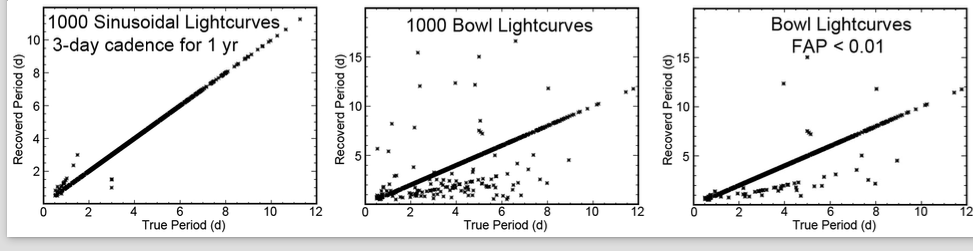
\includegraphics[width=5.32in]{figs/starFormation/tts1.pdf}
 \caption{Recovered period vs. true period for a sample of sinusoidal (left),
bowl-shaped (middle) and bowl-shaped with False Alarm Probability $<$ 0.01 (right),
assuming a 3-day cadence and one year of observing. What appears as a solid line are the
individual points with periods that are recovered correctly. The bowl-shaped curves are
more difficult to recover than the sinusoids, but the method is highly successful in both cases.}
   \label{tts1}
\end{center}
\end{figure}

\begin{figure}[b]
\vspace*{1.0 cm}
\begin{center}
 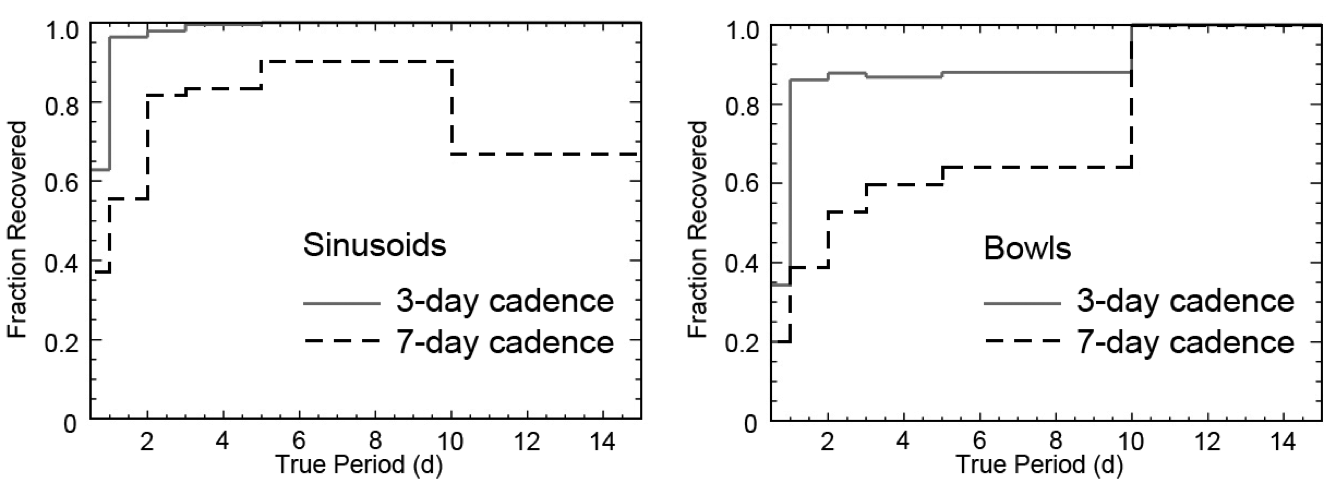
\includegraphics[width=5.32in]{figs/starFormation/tts2.pdf}
 \caption{ Fraction of periods recovered correctly for sinusoidal (left) and bowl light curves (right) for
3-day (solid line) and 7-day (dashed line) cadences over an observing period of one year.
A 3-day cadence is significantly better than a 7-day one. Over 98\%\ of sinusoidal, and 86\%\ of bowl
light curve periods are recovered successfully with the 3-day cadence. The percentages drop to about
82\%\ and 59\%\, respectively, for the 7-day cadence.
}
   \label{tts2}
\end{center}
\end{figure}

\begin{figure}[b]
\vspace*{1.0 cm}
\begin{center}
 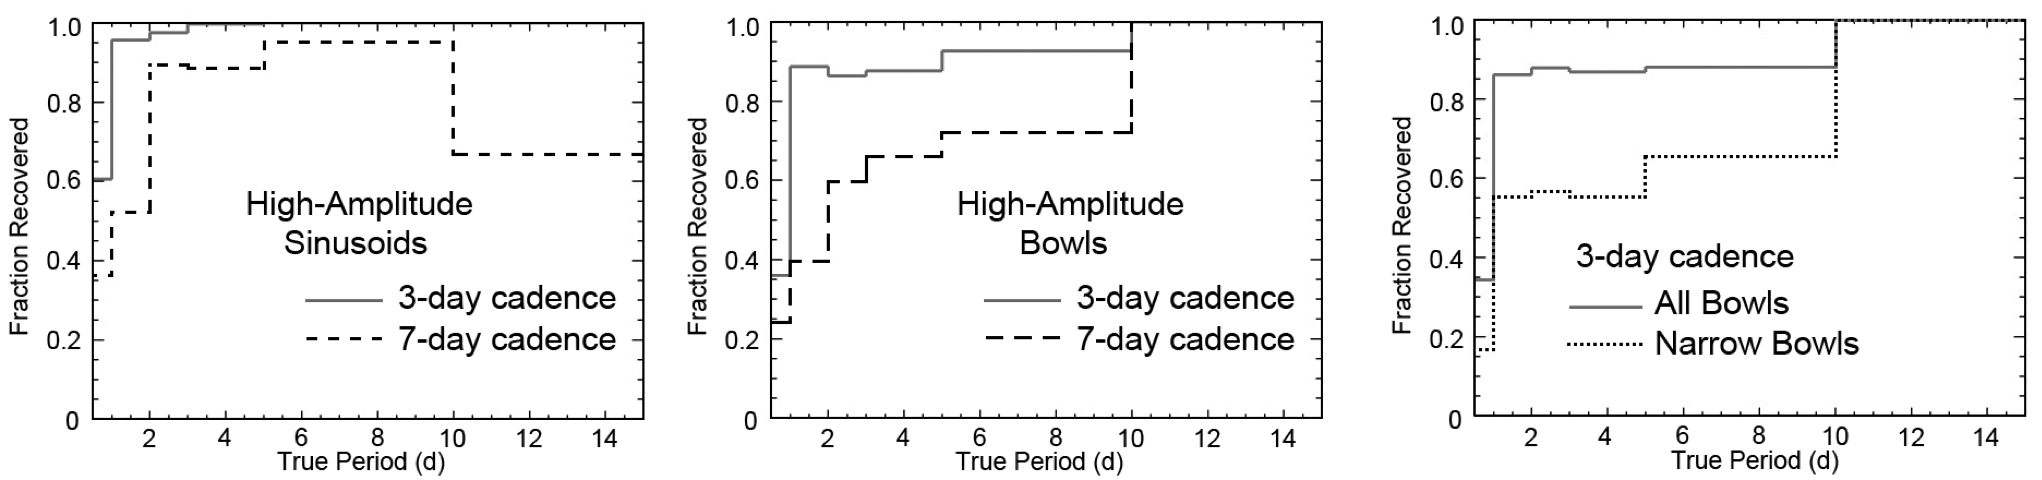
\includegraphics[width=5.32in]{figs/starFormation/tts3.pdf}
 \caption{Left and center: Same as Fig 2 but restricting the sample to amplitudes greater than 0.1 mag. The
method is only marginally more successful with the larger amplitude objects than it is with the entire sample.
Right: The narrowest 278 bowls have a significantly higher error rate than the entire sample does.
}
   \label{tts3}
\end{center}
\end{figure}

Overall, standard cadences of once every few days should suffice
to find most periodic T-Tauri stars that have periods $\gtrsim$ 3 days.
A dedicated campaign to observe star-forming regions
at time intervals of an hour or less is required to capture the shorter-period systems.
The r-filter should suffice for most objects, though some benefit will be had
by going to z to allow the more heavily-extincted sources to be observed.

{\bf C. Period Recovery for cTTs}

Complex irregular variations in cTTs lightcurves make it much more difficult,
and in many cases impossible to
recover periods in these systems. While sparse coverage of one observation every
few days is adequate for identifying sudden changes from accretion events, these
events to a large degree overwhelm low-amplitude periodic signatures. Even when
period searches yield a low false-alarm probability, the results are not necessarily
reliable. Results from Palomar Transient Factory surveys in the North American
Nebula \citep{Findeisen2013} and with Spitzer
\citep{Cody2014}
reveal several types of both short- and long-term variations including both bursting and
fading.  These observations emphasize how important it will be to have some
dense phase coverage as a reality check to ensure the reliability of
any periods recovered from sparse data in these objects, as well as to
follow the short-term variations that characterize accreting systems.

{\bf D. Discovery, Accretion and Extinction Events}

As we indicated above, any
cadence will uncover FU Ori and EX Ori events in all filters.
Periodic extinction events follow the same restrictions and
have the same requirements as rotational periods described in subsection B.

In order to assess the ability of LSST to identify and classify
eruptive variables (FUor/EXor), we construct
\autoref{table:pseudoForExor}, which shows a possible Figure of Merit for the
recovery by LSST of the distribution of EXor high-state duration in
outburst.

\begin{table}
\small
\begin{tabular}{c p{12cm}}
& {\it Figure of Merit for recovery of EXor high--state duration distribution}\\
\hline
1.  & Produce ASCII lightcurve for eruptive outburst \\
2.  & Initialise large array to store the maps of fraction detected as a function of duration and amplitude. \\
2.  & for {\it duration T} in range \{min, max\}:  \\
3.  & ~~~~ for {\it amplitude A} in range \{min, max\}: \\
4.  & ~~~~~~~~~~ run {\tt mafContrib/transientAsciiMetric} \\
5.  & ~~~~~~~~~~ store the spatial map of the fraction detected for this (A, T) pair \\
6.  & Initialise master arrays to hold the run of duration distribution measurements.\\
7. & Produce distribution of high--state durations and amplitudes from which the simulations will be drawn. \\
8.  & for {\it iDraw} in range \{1, nDraws\}:\\
9.  & ~~~~ construct model population with input duration distribution \\
10.  & ~~~~ Apply the stored metrics from 2-5 to measure fraction recovered \\
11.  & ~~~~ Characterize the duration distribution for this draw \\
12. & ~~~~ Fill the {\it iDraw}'th entry in the master arrays. \\
13. & {\bf FoM 1:} Compute the median and variance of the upper/lower quintiles. \\
14. & {\bf FoM 2:} Evaluate the bias between recovered and input high-state duration. \\
\hline
\end{tabular}
\caption{Steps for Figure of Merit recovering the distribution
  for the duration of EXor high states.}
\label{table:pseudoForExor}
\end{table}

% --------------------------------------------------------------------

\subsection{Summary and Recommendations}
\label{sec:\secname:discussion}

{\bf Performance for Nominal Cadences}

Nominal cadences that return to a star-forming region every 3-4 days
will suffice to determine rotation periods for $\sim$ 90\%\ of the
young stars within the magnitude limits of LSST.
These cadences are also adequate to detect major episodic
accretion events like FU Ori's and EX Ori's. However, a more focused
annual campaign of about a week duration is necessary to optimize
period recovery and angular momentum studies of young stars.

{\bf The Need for Annual Dense Coverage of a Few Selected Regions}

Occasional dense coverage of targeted regions is the only way to
get quantitative information on short-term accretion and flare
activity.  Dense coverage also removes degeneracies
for periodic variables that have periods less than a day, and is
the only way to provide a sanity check on any periods recovered for
cTTs, which have complex irregular light variations.
Comparing longevities of starspots across the mass ranges of young
stars requires two well-sampled lightcurves separated by large
time intervals.  The embedded and Classical T Tauri stars also undergo
significant and rapid color changes due to both accretion processes
and extinction variations, so it is important
to include multiple filters in any dense coverage campaign.

These goals can be accomplished by having a week every year where
one or more selected fields are observed once every 30 minutes in u, r and z.
A young star with a 2-day period sampled every 30 minutes provides a
data point every 0.01 in phase. For the best-case scenario, observing for 7 nights
and 10 hours per night would yield 140 photometric points in each filter.
Depending on the period aliasing, this coverage should populate the
phases well enough to identify most of the large starspots on the stellar photospheres.

At the beginning of LSST operations we argue that a targeted test field
be observed in this manner to illustrate what can be done with LSST in this mode.
Combining a densely-packed short-interval
dataset with a sparse but long baseline study maxmizes the scientific return
for both methods, and allows LSST to address all of the accretion and
rotational variability associated with young stars.

\subsection{Conclusions}
\begin{description}
\item[Q1:] {\it Does the science case place any constraints on the
tradeoff between the sky coverage and coadded depth? For example, should
the sky coverage be maximized (to $\sim$30,000 deg$^2$, as e.g., in
Pan-STARRS) or the number of detected galaxies (the current baseline 
of 18,000 deg$^2$)?}
%
\item[A1:] 
Most young stars congregate into clusters in specific regions, though there is an older
population that is more distributed. The vast majority are within $\sim$ 25 degrees of the
galactic plane. As long as that swath of sky is covered to the degree possible from Chile,
the survey will provide the young star community with the monitoring capability needed to
identify transient outbursts and to study periodic and aperiodic phenomena in young stars.
While it may be useful to have deep coadded images of some regions, for example, to identify
optical counterparts to X-ray point sources, dust extinction typically limits such efforts
in the optical towards most regions of interest.  Hence, deep coadded frames are a secondary
priority.

\item[Q2:] {\it Does the science case place any constraints on the
tradeoff between uniformity of sampling and frequency of  sampling? For
example, a rolling cadence can provide enhanced sample rates over a part
of the survey or the entire survey for a designated time at the cost of
reduced sample rate the rest of the time (while maintaining the nominal
total visit counts).}

\item[A2:] 
We discussed cadences in some detail above. To obtain the best constraints on periods, a time-intensive
($\sim$ one week/year) campaign on a few selected regions is warranted. Nominal coverage over the
galactic plane will suffice to identify eruptive variables.

\item[Q3:] {\it Does the science case place any constraints on the
tradeoff between the single-visit depth and the number of visits
(especially in the $u$-band where longer exposures would minimize the
impact of the readout noise)?}

\item[A3:] 
This item is discussed in section A above. In young stars, the u-band is particularly useful
as a measure of accretion. At the same time, for period determinations, denser cadences produce
fewer problems with aliasing for the typical young star variable with a rotation period between
a day and two weeks.

\item[Q4:] {\it Does the science case place any constraints on the
Galactic plane coverage (spatial coverage, temporal sampling, visits per
band)?}

\item[A4:] 
A nominal sampling of once every few days will suffice to identify interesting
eruptive variables as long as the galactic plane coverage is good (item A1).
However, a sparse temporal sampling such as this will make it difficult to interpret
the lightcurves of the tens of thousands of T Tauri stars observed by LSST. A single
week's campaign of dense sampling, e.g., 2-3 times per night, of targeted regions
will greatly improve our ability to separate periodic variables from aperiodic ones. 
Knowing the rotation periods of thousands of young stars within a given star forming
region will be a major contribution that LSST makes to this field of research. Such data
will allow us to learn how angular momentum is distributed among newborn
stars, whether it changes with mass and location in the cloud, 
and how it varies as the stars age. 

\item[Q5:] {\it Does the science case place any constraints on the
fraction of observing time allocated to each band?}

\item[A5:] 
In the case we made above for dense sampling, we argued for z, r, and u. The
u-band allows us to follow mass accretion variability, while r and z (for most
objects) will be dominated by photospheric flux. The r-z color is an important
constraint for models of star spots. More colors are always useful, but having
a photospheric color index plus one accretion measure are the science drivers 
for filter choices. Once u, r, and z are observed, having higher cadences
is preferable to having more bands.
The exposure times and magnitudes for typical objects are described in section A
above.

\item[Q6:] {\it Does the science case place any constraints on the
cadence for deep drilling fields?}

\item[A6:] 
Absolutely. We argue in the `Summary and Recommendations' section above
for the advantages of a single week of denser monitoring for specific
regions, with the goal of having several observations per night, separated
in time by at least an hour from one another. The goal here is to provide
some basis in reality for interpreting the irregular lightcurves of young
stars, which also typically have a periodic component. Depending on the longevity of
the star spots, a period might be obvious in high-cadence data taken over
a week, but disappear over a year if some spots vanish and others form. 

\item[Q7:] {\it Assuming two visits per night, would the science case
benefit if they are obtained in the same band or not?}

\item[A7:] 
If the data are taken in the same band
it means better sampling for periods. With different bands it means a lightcurve in two bands,
which is also useful. It's probably a wash, and we can follow whatever the drivers are for the
other science cases of LSST.

\item[Q8:] {\it Will the case science benefit from a special cadence
prescription during commissioning or early in the survey, such as:
acquiring a full 10-year count of visits for a small area (either in all
the bands or in a  selected set); a greatly enhanced cadence for a small
area?}

\item[A8:] 
Yes, definitely. We ought to see what we can get out of a dedicated week-long
LSST cadence on specific regions. If the results are impressive we follow up 
on different regions every year (or even return to the same regions).

\item[Q9:] {\it Does the science case place any constraints on the
sampling of observing conditions (e.g., seeing, dark sky, airmass),
possibly as a function of band, etc.?}

\item[A9:] 

Better seeing helps with unresolved binaries and for regions where contamination comes
into play, for example, in the plane but away from dark clouds. Some of the fainter objects
will be affected if the Moon is very bright and close. However generally these constraints
are probably in a 'typical' category and will not affect the design of the survey.

\item[Q10:] {\it Does the case have science drivers that would require
real-time exposure time optimization to obtain nearly constant
single-visit limiting depth?}

\item[A10:] 
No.

\end{description}

% ====================================================================

% bibtems need pushing into the relevant file!

%Hartmann \& Kenyon 1996, ARA\&A, 34, 207 \\
%Herbig et al. 2001, PASP, 113, 1547 \\
%Herbig 1977, ApJ, 217, 693 \\
%Aspin et al. 2009, ApJ, 692L, 67 \\
%Hodapp et al. 1996, ApJ, 468, 861 \\
%McGehee et al. 2004, ApJ, 616, 1058 \\

%\bibitem[Affer et al. (2013)]{Affer13}
%{Affer, L., Micela, G., Favata, F., Flaccomio, E., \& Bouvier, J.} 2013
%\textit{MNRAS}, 430, 1433

%\bibitem[Alencar al. (2010)]{CoRoT}
%{Alencar, S. H. P. et al.} 2010,
%\textit{A\&A}, 519, A88

%\bibitem[Cody al. (2014)]{cody14}
%Cody, A., et al.
%{Cody, A. et al.} 2014,
%\textit{AJ}, 147, 82

%\bibitem[Grankin al. (2008)]{ROTOR}
%\bibitem[Findeisen al. (2013)]{findeisen13}
%Findeisen, K., Hillenbrand, L., Ofek, E., Levitan, D., Sesar, B., Laher, R., \& Surace, J.
%{Findeisen, K. et al.} 2013,
%\textit{ApJ}, 768, 93

%\bibitem[Grankin al. (2008)]{ROTOR}
%{Grankin, K. N., Bouvier, J., Herbst, W., \& Melnikov, S. Yu.} 2008,
%\textit{A\&A}, 479, 827

%\bibitem[Horne \& Baliunas (1986)]{Scargle}
%{Horne, J. H. \& Baliunas, S.} 1986, \textit{ApJ}, 302, 757

\navigationbar
